\documentclass[presentation]{subfiles}

\begin{document}
\begin{frame}{Planes, Trains, and Automobiles}
  \begin{columns}
  \only<1,4->{
  \only<1>{
  \begin{column}{0.5\textwidth}
  \centering
  Trains
  % \begin{figure}
  %   \begin{overlayarea}{\textwidth}{4cm}
  %   \begin{minipage}[c][4cm]{\textwidth}
      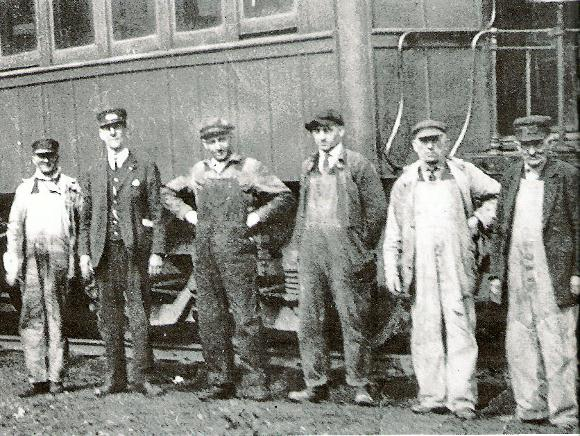
\includegraphics[width=\textwidth]{figures/photo/train_workers.jpg}
      \end{column}
  }
  \only<4->{

  \begin{column}{0.33\textwidth}
  \centering
  Trains
  % \begin{figure}
  %   \begin{overlayarea}{\textwidth}{4cm}
  %   \begin{minipage}[c][4cm]{\textwidth}
      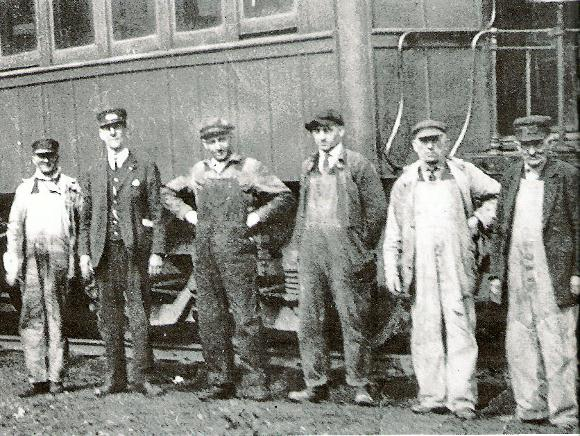
\includegraphics[width=\textwidth]{figures/photo/train_workers.jpg}
    % \end{minipage}
    % \end{overlayarea}
    % \end{figure}
\end{column}
}

\only<1>{
    \begin{column}{0.5\textwidth}
      \begin{itemize}
        \item ``Efficiency experts'' measured how long it would take to do various jobs\par
        \scriptsize{\textcite{doi:10.2307/1883615}\par}\normalsize{}
        \item These measurements would be used to assign values for each specific task\par
        \scriptsize{\textcite{american1921problem}\par}\normalsize{}
        % \item Train engineers instituted ``The Fix'' to correct perceived unfairness\par
        % \scriptsize{\textcite{roy1954efficiency}\par}\normalsize{}
      \end{itemize}
    \end{column}
  }
}

  \only<2,4->{
    \only<2>{
      \begin{column}{0.25\textwidth}
      \begin{itemize}
        \item Consolidating and training workers (\emph{Fordism})\par
        \scriptsize{\textcite{schoenberger1988fordism,tolliday1986between}\par}\normalsize{}
        % \item Fordism, Taylorism, and Scientific Management in full force
      \end{itemize}
      \end{column}
    }

  \only<2>{
    \begin{column}{0.5\textwidth}
    \centering
      Automobiles
      % \begin{figure}
      %   \begin{overlayarea}{\textwidth}{4cm}
      %   \begin{minipage}[c][4cm]{\textwidth}
          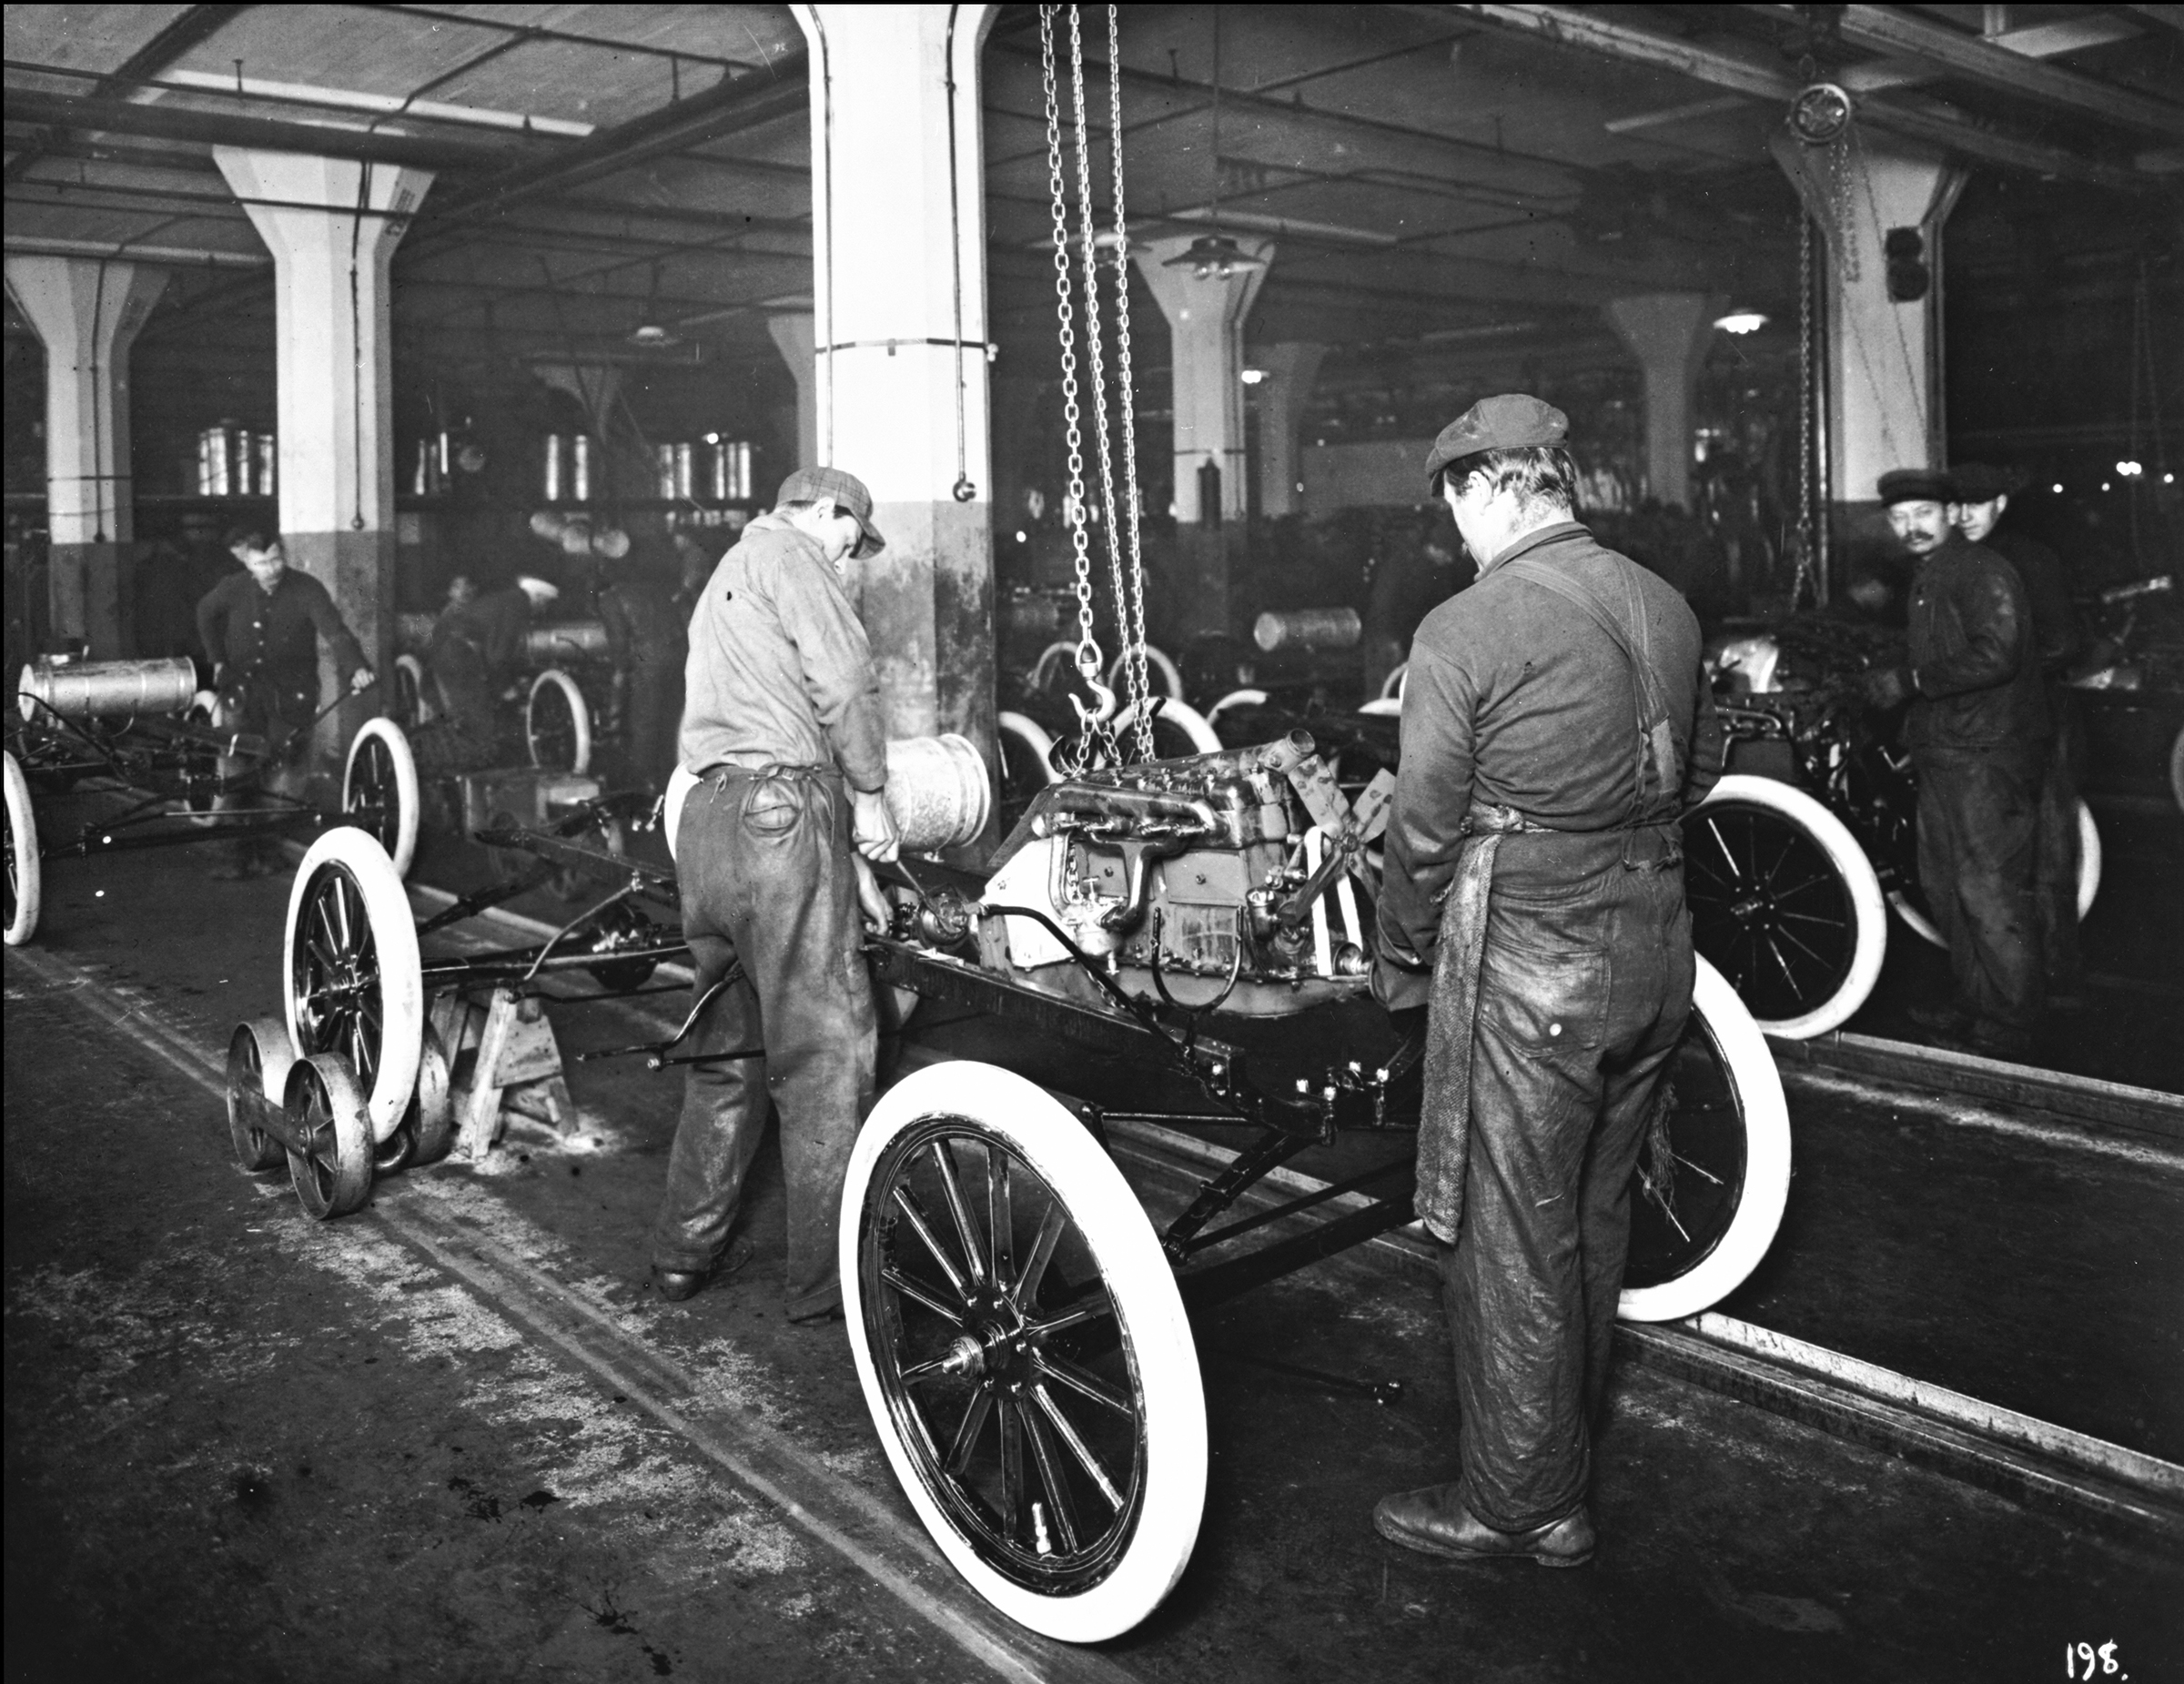
\includegraphics[width=\textwidth]{figures/photo/ford_assembly_line.jpg}
      %   \end{minipage}
      %   \end{overlayarea}
      % \end{figure}
  \end{column}
  }
  \only<4->{
  \begin{column}{0.33\textwidth}
    \centering
      Automobiles
      % \begin{figure}
      %   \begin{overlayarea}{\textwidth}{4cm}
      %   \begin{minipage}[c][4cm]{\textwidth}
          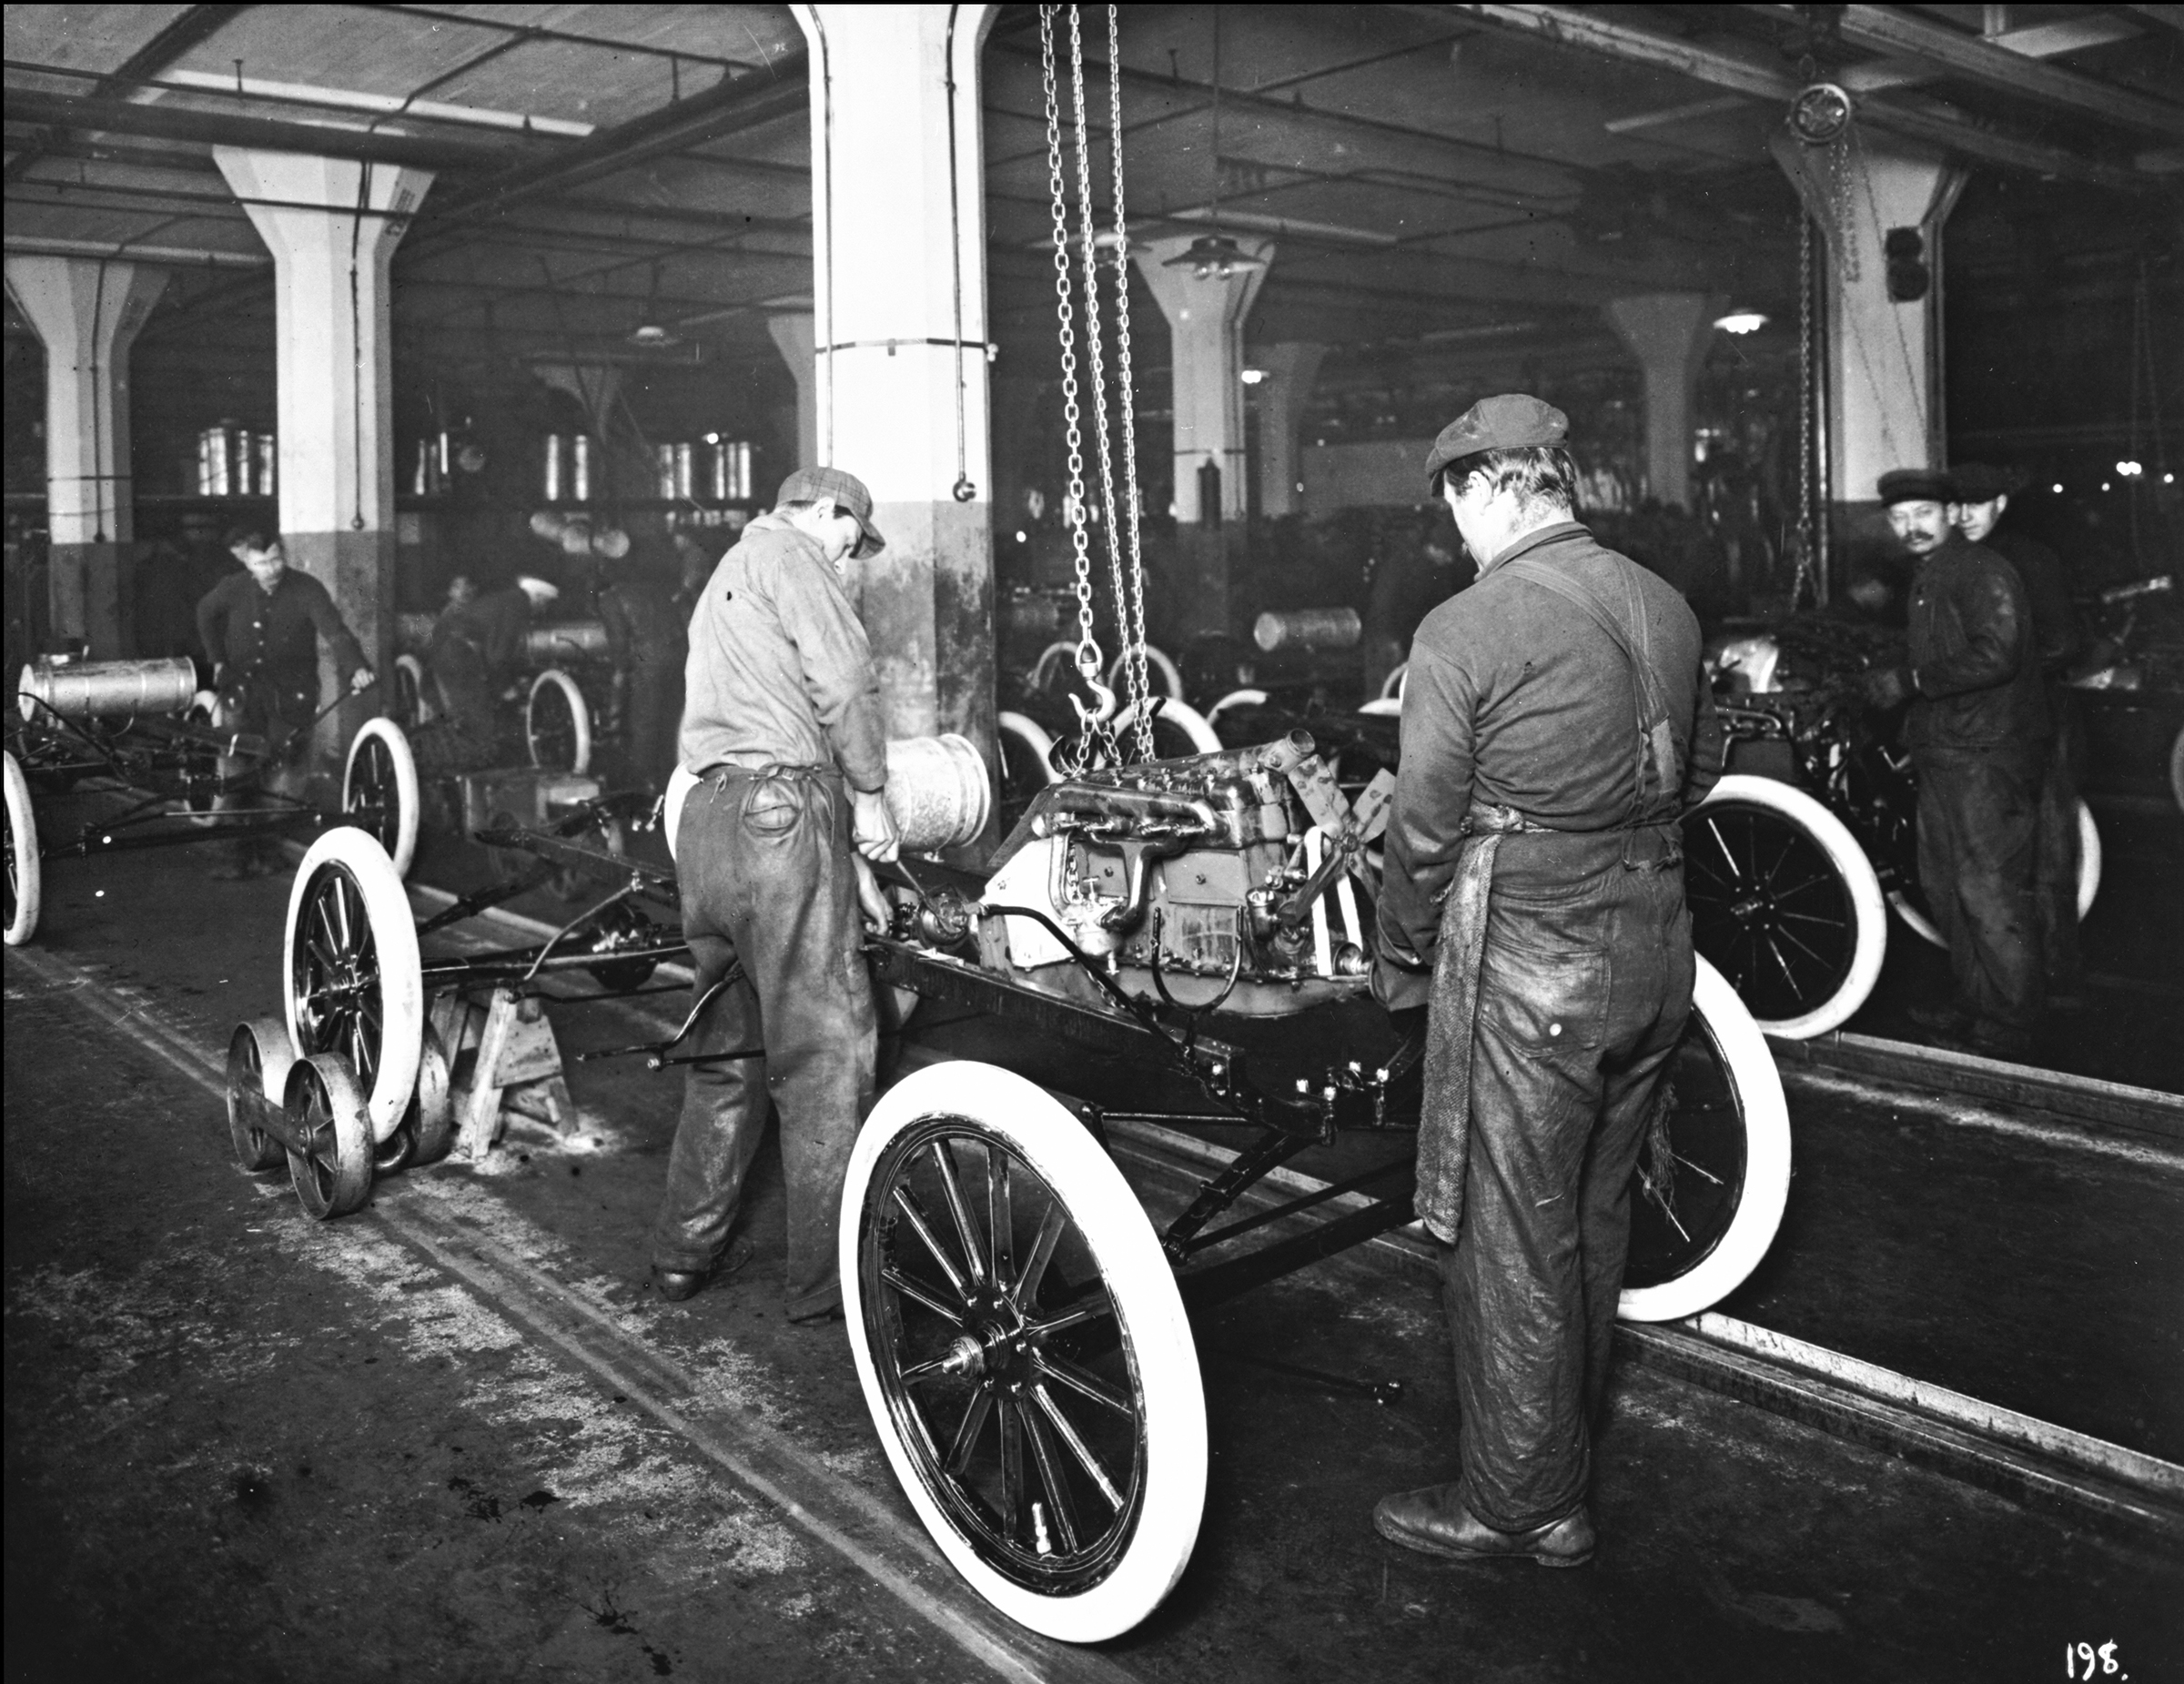
\includegraphics[width=\textwidth]{figures/photo/ford_assembly_line.jpg}
      %   \end{minipage}
      %   \end{overlayarea}
      % \end{figure}
  \end{column}
  }
  
  \only<2>{
    \begin{column}{0.25\textwidth}
    \begin{itemize}
        \item Measuring and evaluating workers by very carefully defined instructions (\emph{Taylorism})\par
        \scriptsize{\textcite{taylor1914principles}\par}\normalsize{}
      % \item \emph{Manufacturing} proved amenable
      %       to assembly line processes.
    \end{itemize}
    \end{column}
  }
}

  \only<3->{
    \only<3>{
      \begin{column}{0.5\textwidth}
      \begin{itemize}
        \item Men drafted during World War II
        \item Factories turned to a new workforce who had neither conventional training nor experience
        \item \textbf{Specialized training and assignment}
      \end{itemize}
      \end{column}
    }
    \only<3>{
  \begin{column}{0.5\textwidth}
    \centering
      Planes
      % \begin{figure}
      %   \begin{overlayarea}{\textwidth}{4cm}
      %   \begin{minipage}[c][4cm]{\textwidth}
            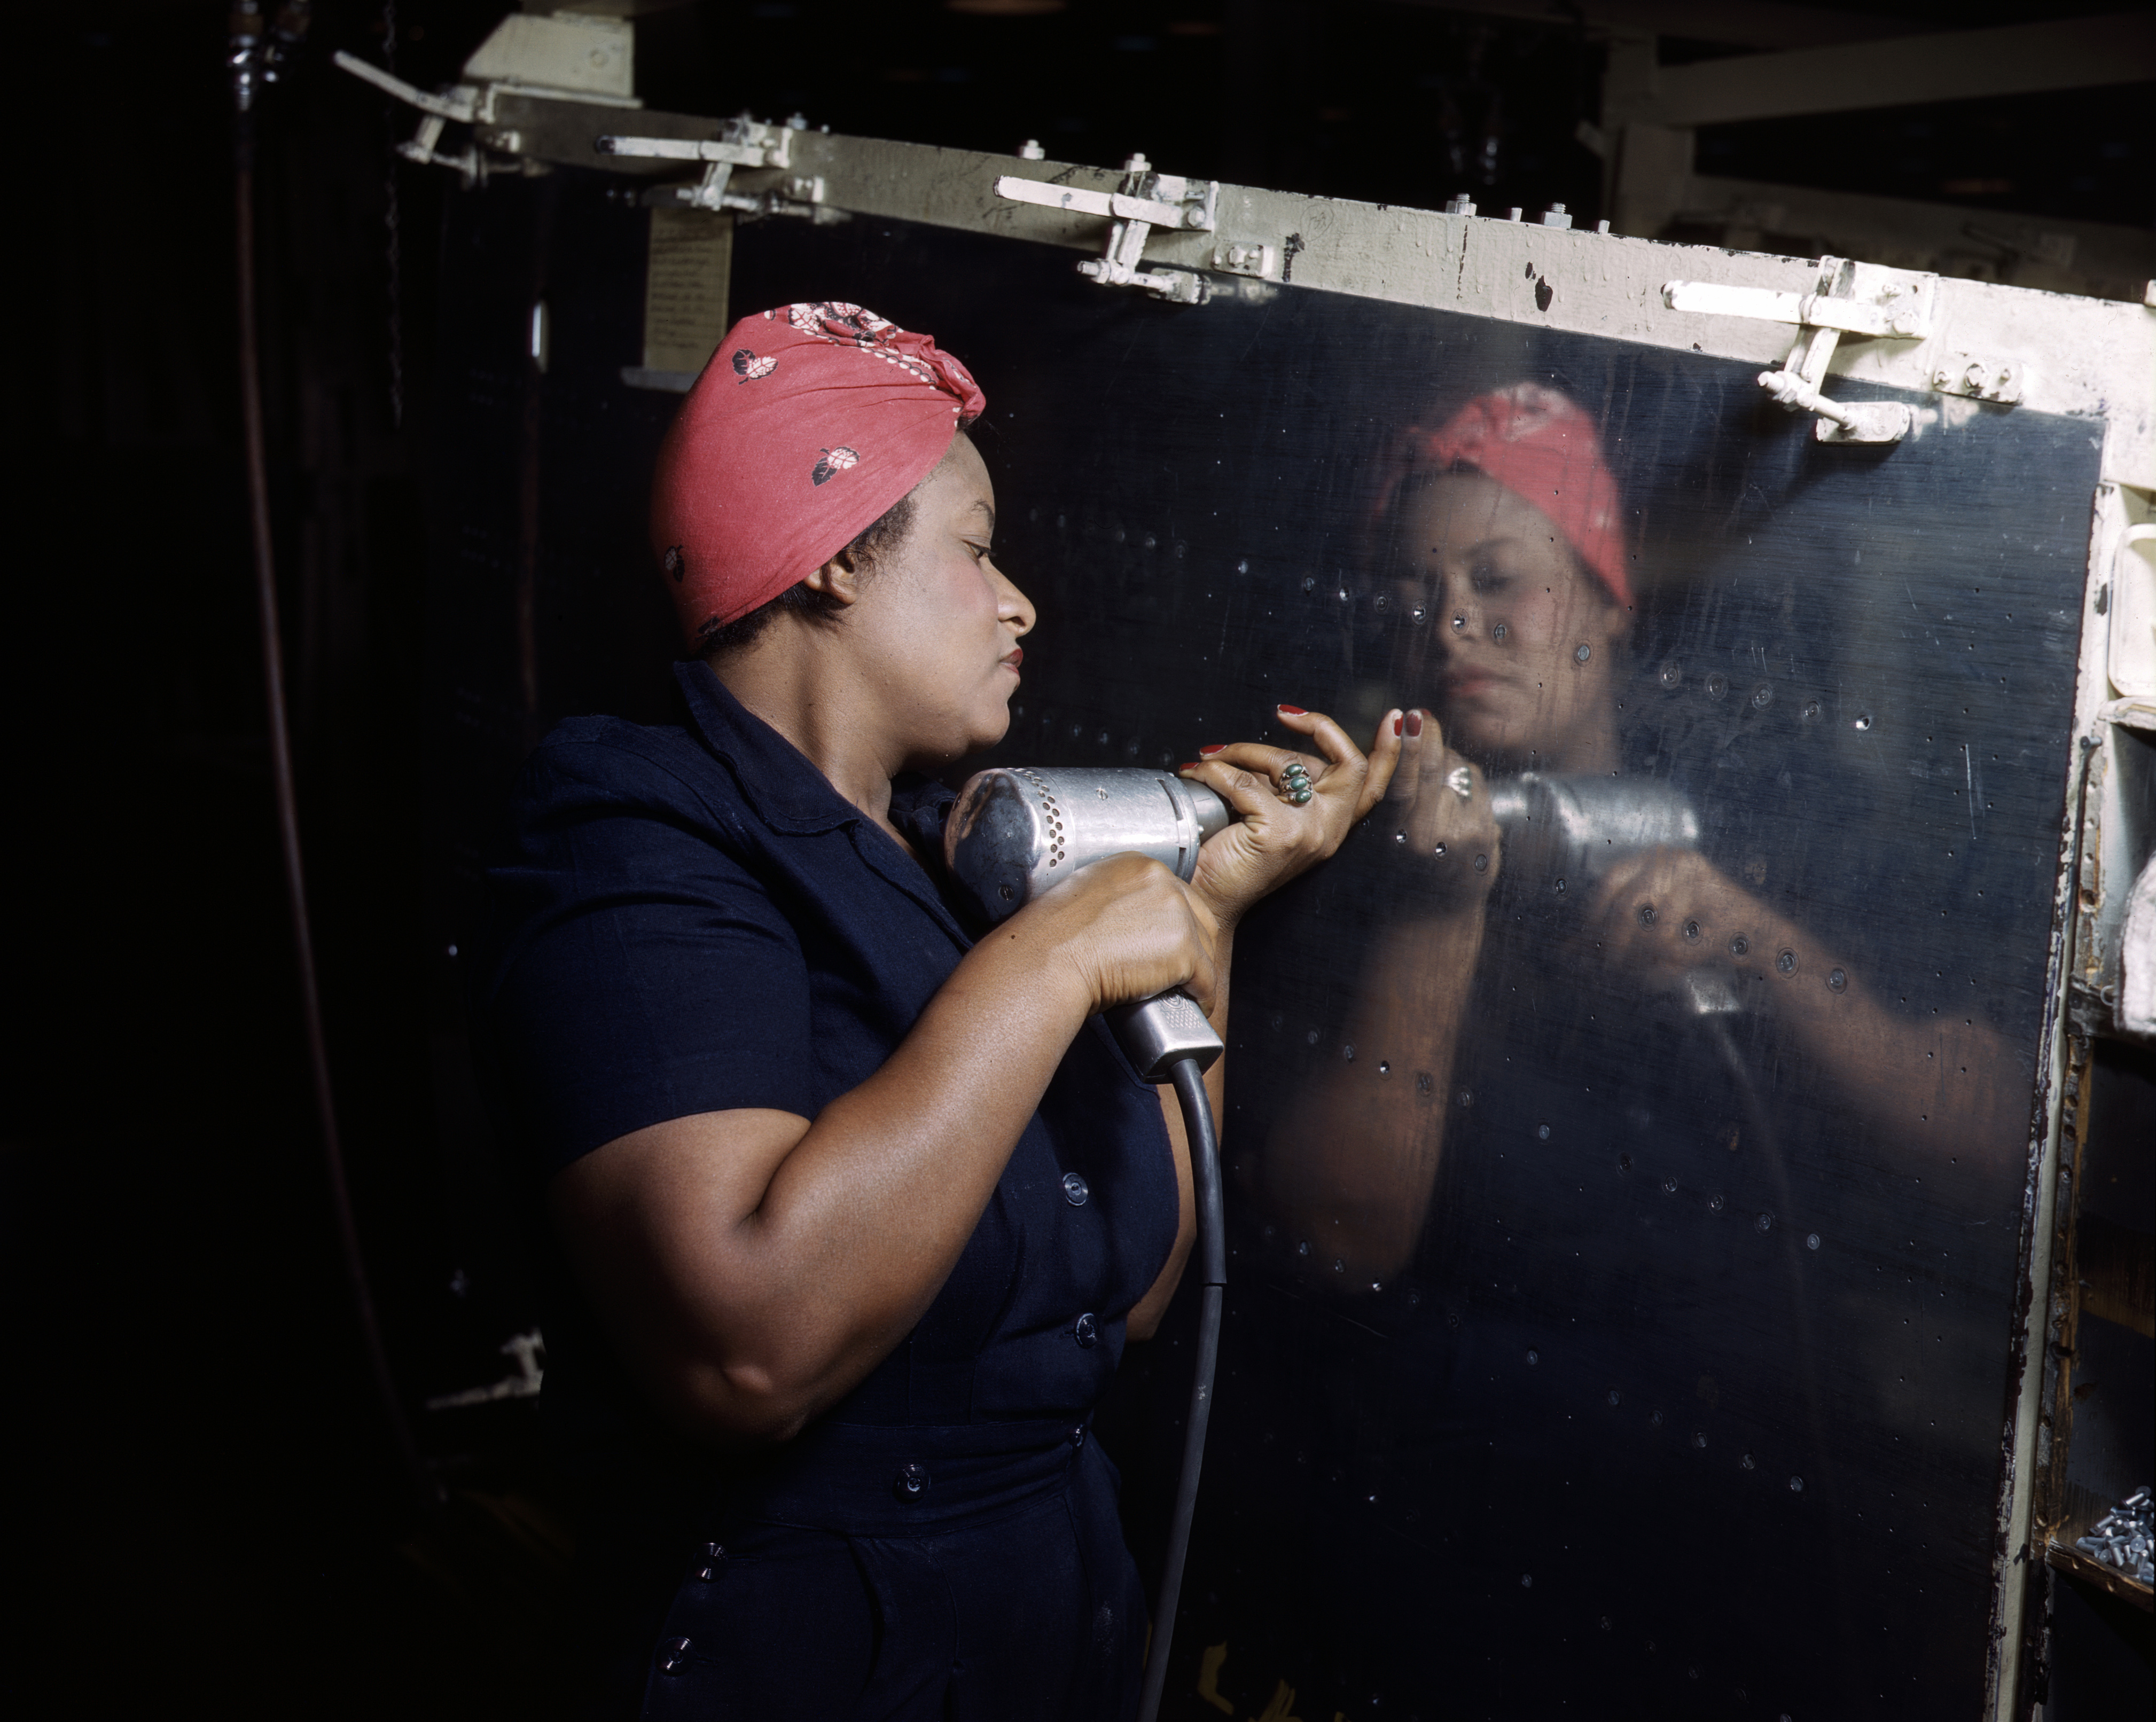
\includegraphics[width=\textwidth]{figures/photo/Rosie_the_Riveter_(Vultee)_DS.jpg}
      % \end{minipage}
      % \end{overlayarea}
      % \end{figure}
  \end{column}
  }
  \only<4->{
  \begin{column}{0.33\textwidth}
    \centering
      Planes
      % \begin{figure}
      %   \begin{overlayarea}{\textwidth}{4cm}
      %   \begin{minipage}[c][4cm]{\textwidth}
            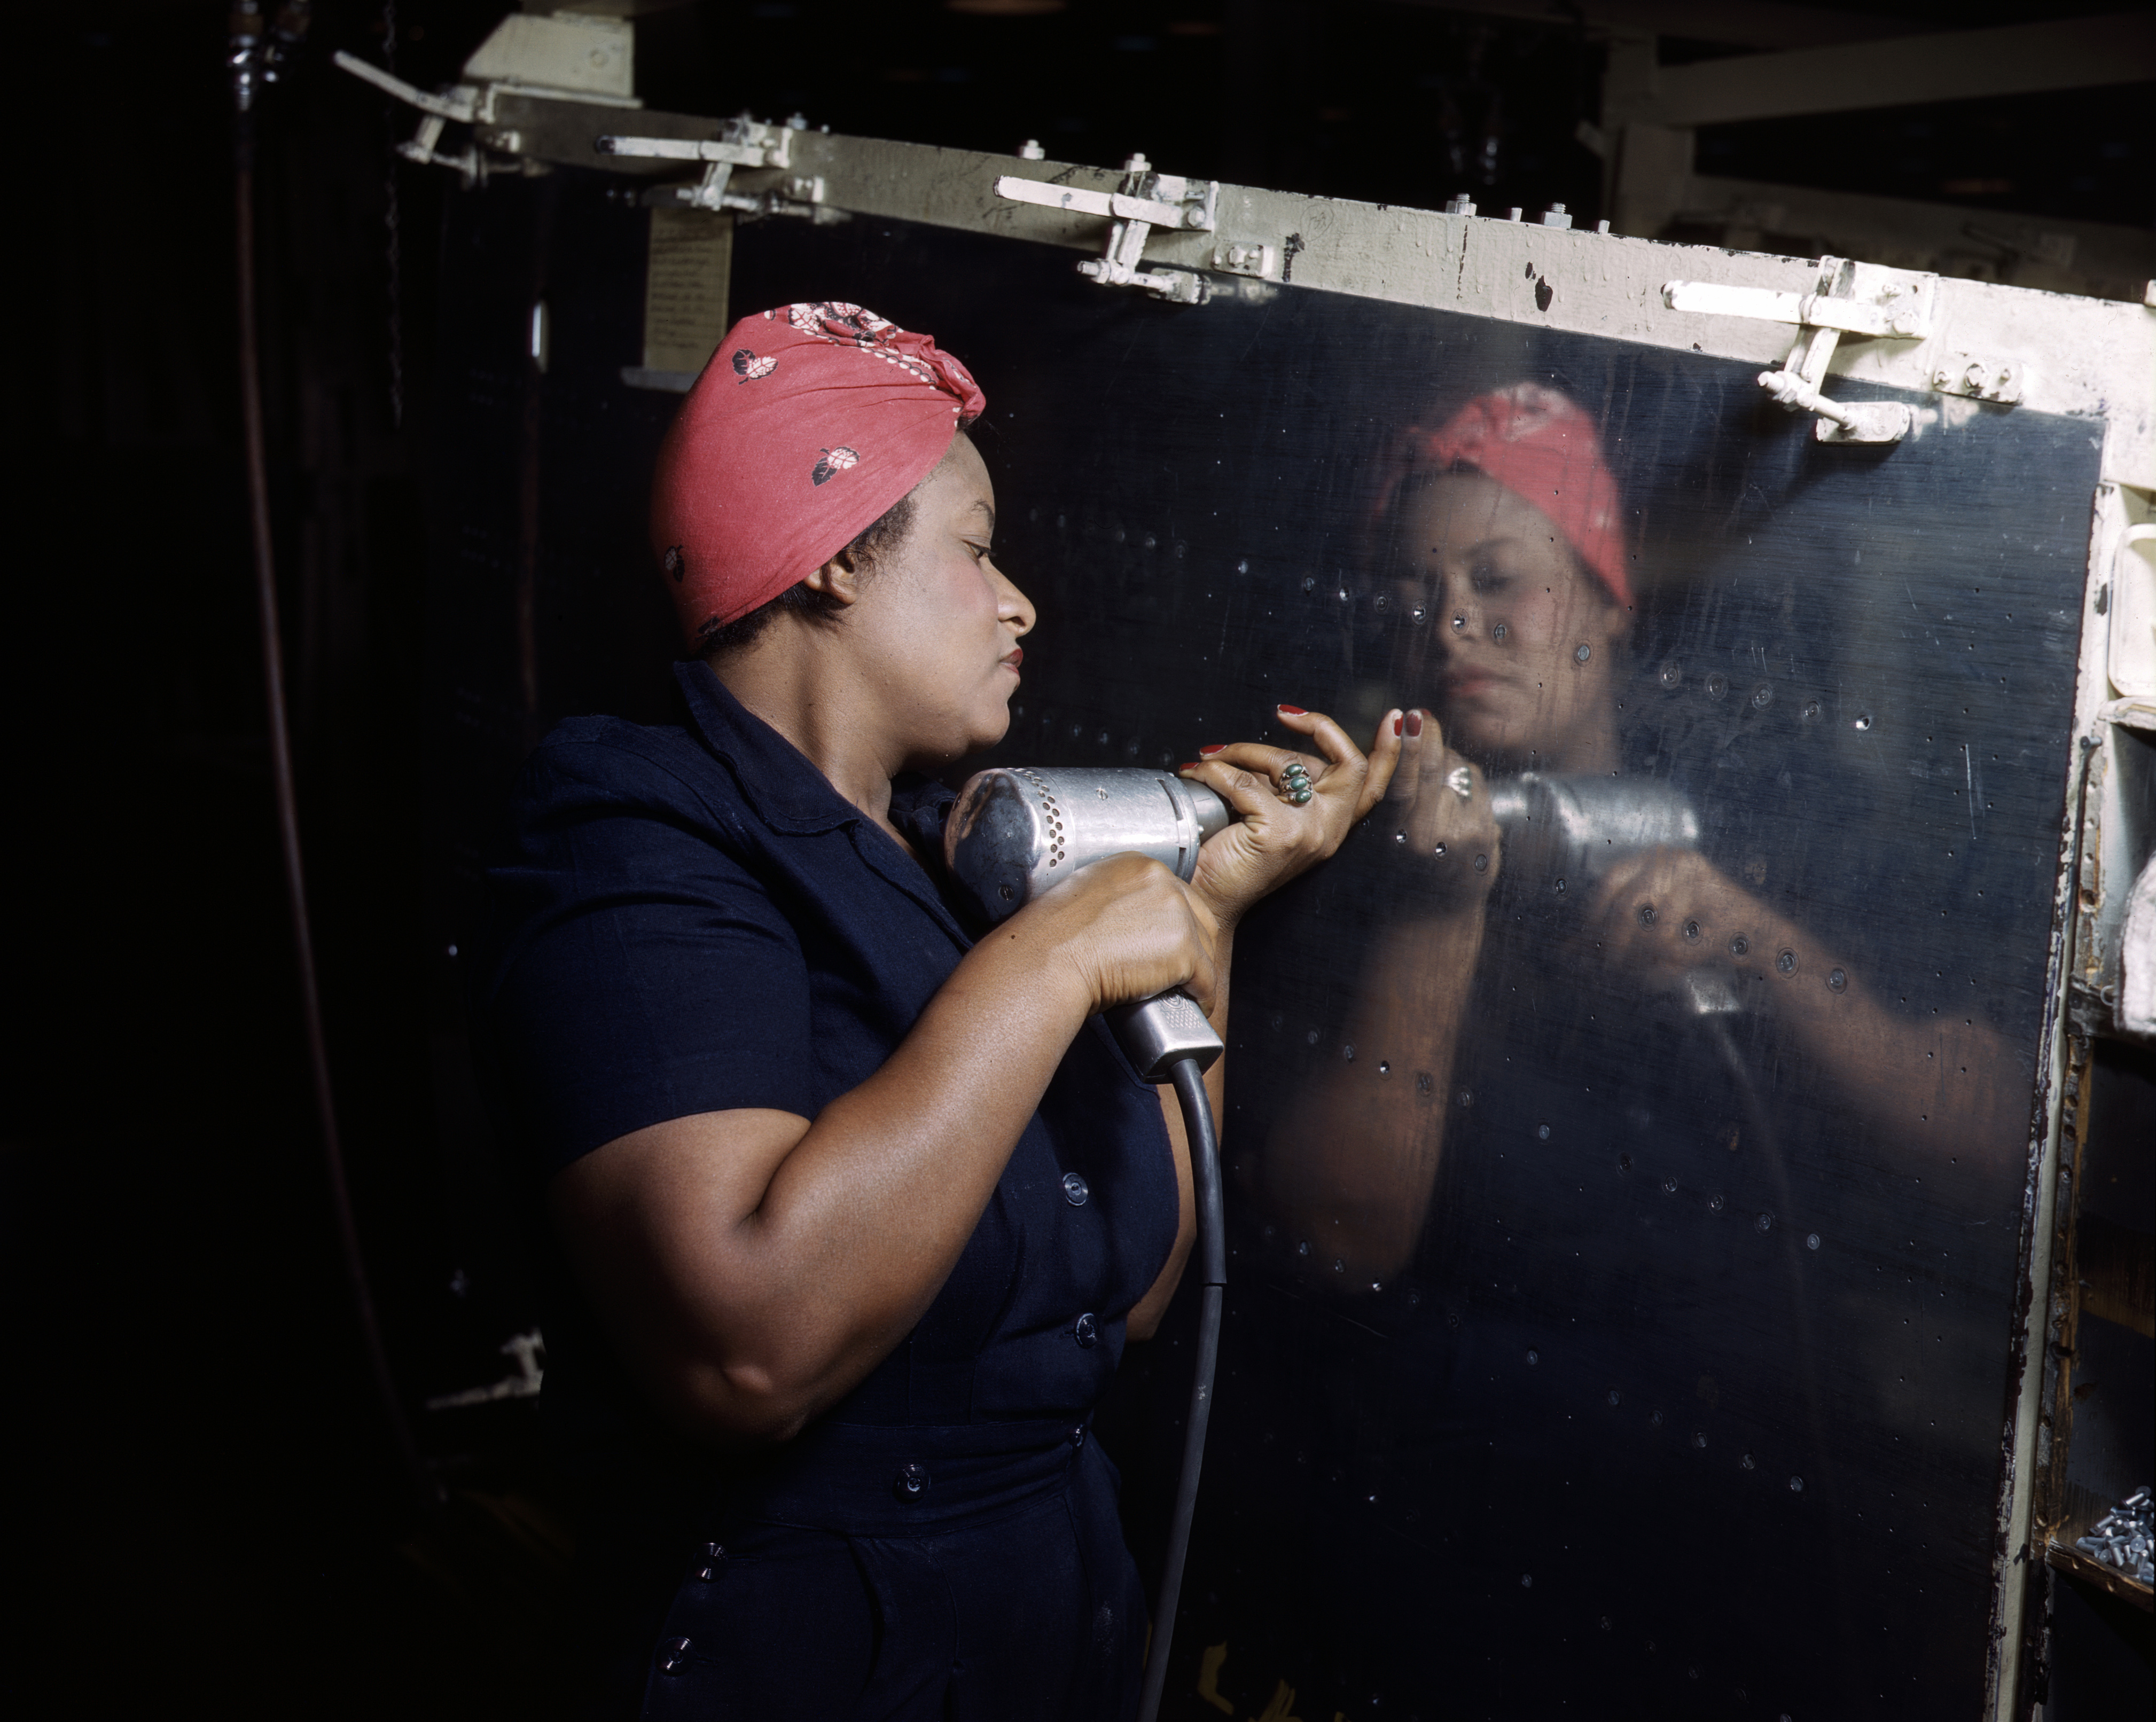
\includegraphics[width=\textwidth]{figures/photo/Rosie_the_Riveter_(Vultee)_DS.jpg}
      % \end{minipage}
      % \end{overlayarea}
      % \end{figure}
  \end{column}
  }
}
  \end{columns}


\end{frame}
\end{document}